\documentclass[main.tex]{subfiles}

\begin{document}
\section{程序运行测试}

\subsection{测试程序}
我按照老师要求,开发以下程序并进行测试:

主程序加载到0x0000\_3000,内容如下:
\inputminted[linenos]{gas}{Project4/p3-test-main-commented.asm}

中断服务程序加载到0x0000\_4180,内容如下:
\inputminted[linenos]{gas}{Project4/p3-test-int-commented.asm}

\clearpage

\subsection{测试方法与结果}

\paragraph{测试方法}
将程序写入FPGA中,进行实机实验。测试软件功能,若功能与预期一致则认为测试成功。

\paragraph{测试结果}

\subparagraph{正确性测试} 动态数码管和$Main$系统频率(CPU主频)均设为1kHz,写入FPGA后,可正常实现预期中的自动计时、置数后重置以及按下重置按钮后重置等功能。系统外特性几乎与理想完全一致,只是计时略慢于实际时间。

考虑到CPU主频仅有1kHz,存在由于执行指令导致延迟的情况,整体表现与预期相符。

\subparagraph{提高主频尝试} 验证系统正确性后,我尝试修改分频器和主程序,以实现外特性不变而提高CPU主频的效果。经过多次尝试,我最高尝试出2MHz主频下不会出错。

频率再高时会出现高位显示异常的bug,推测是由于每一个周期时间过短,寄存器存取或某模块计算较慢导致的出错,与预期相符。

\begin{figure}[h]
\centering
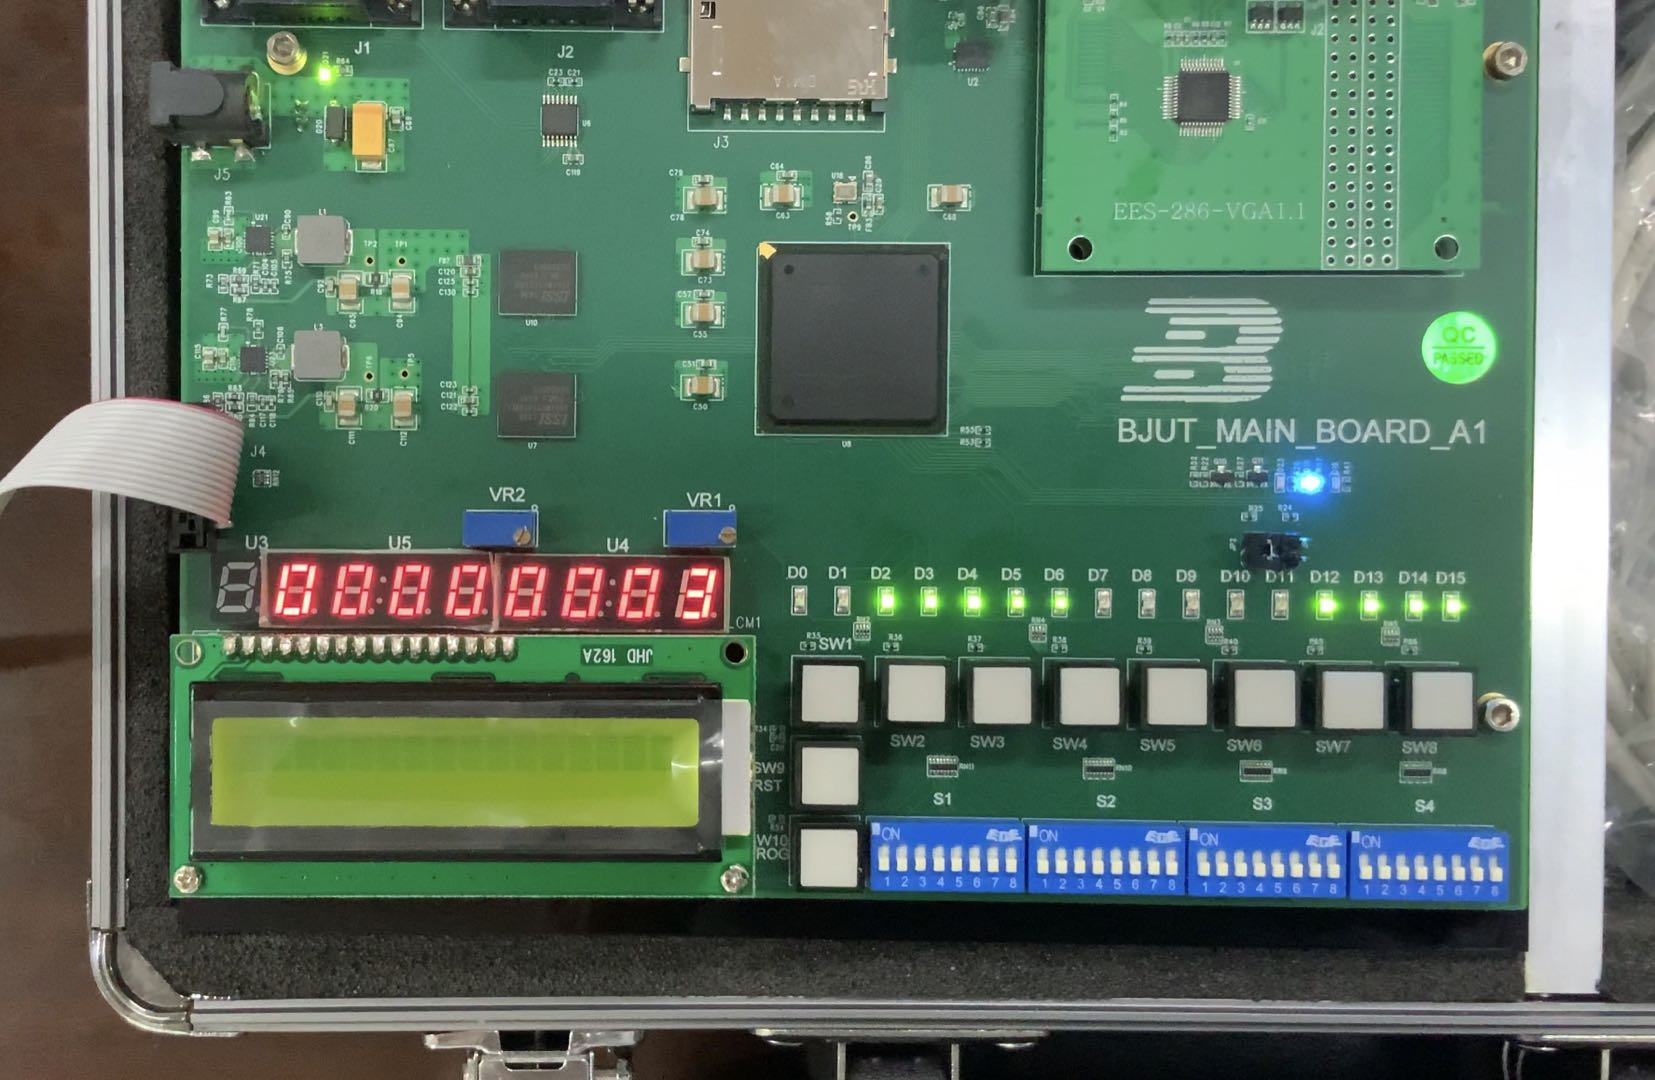
\includegraphics[width=\textwidth]{images/2MHz-add.jpg}
\caption{2MHz下正常运行-从零计数}
\end{figure}

\begin{figure}[h]
\centering
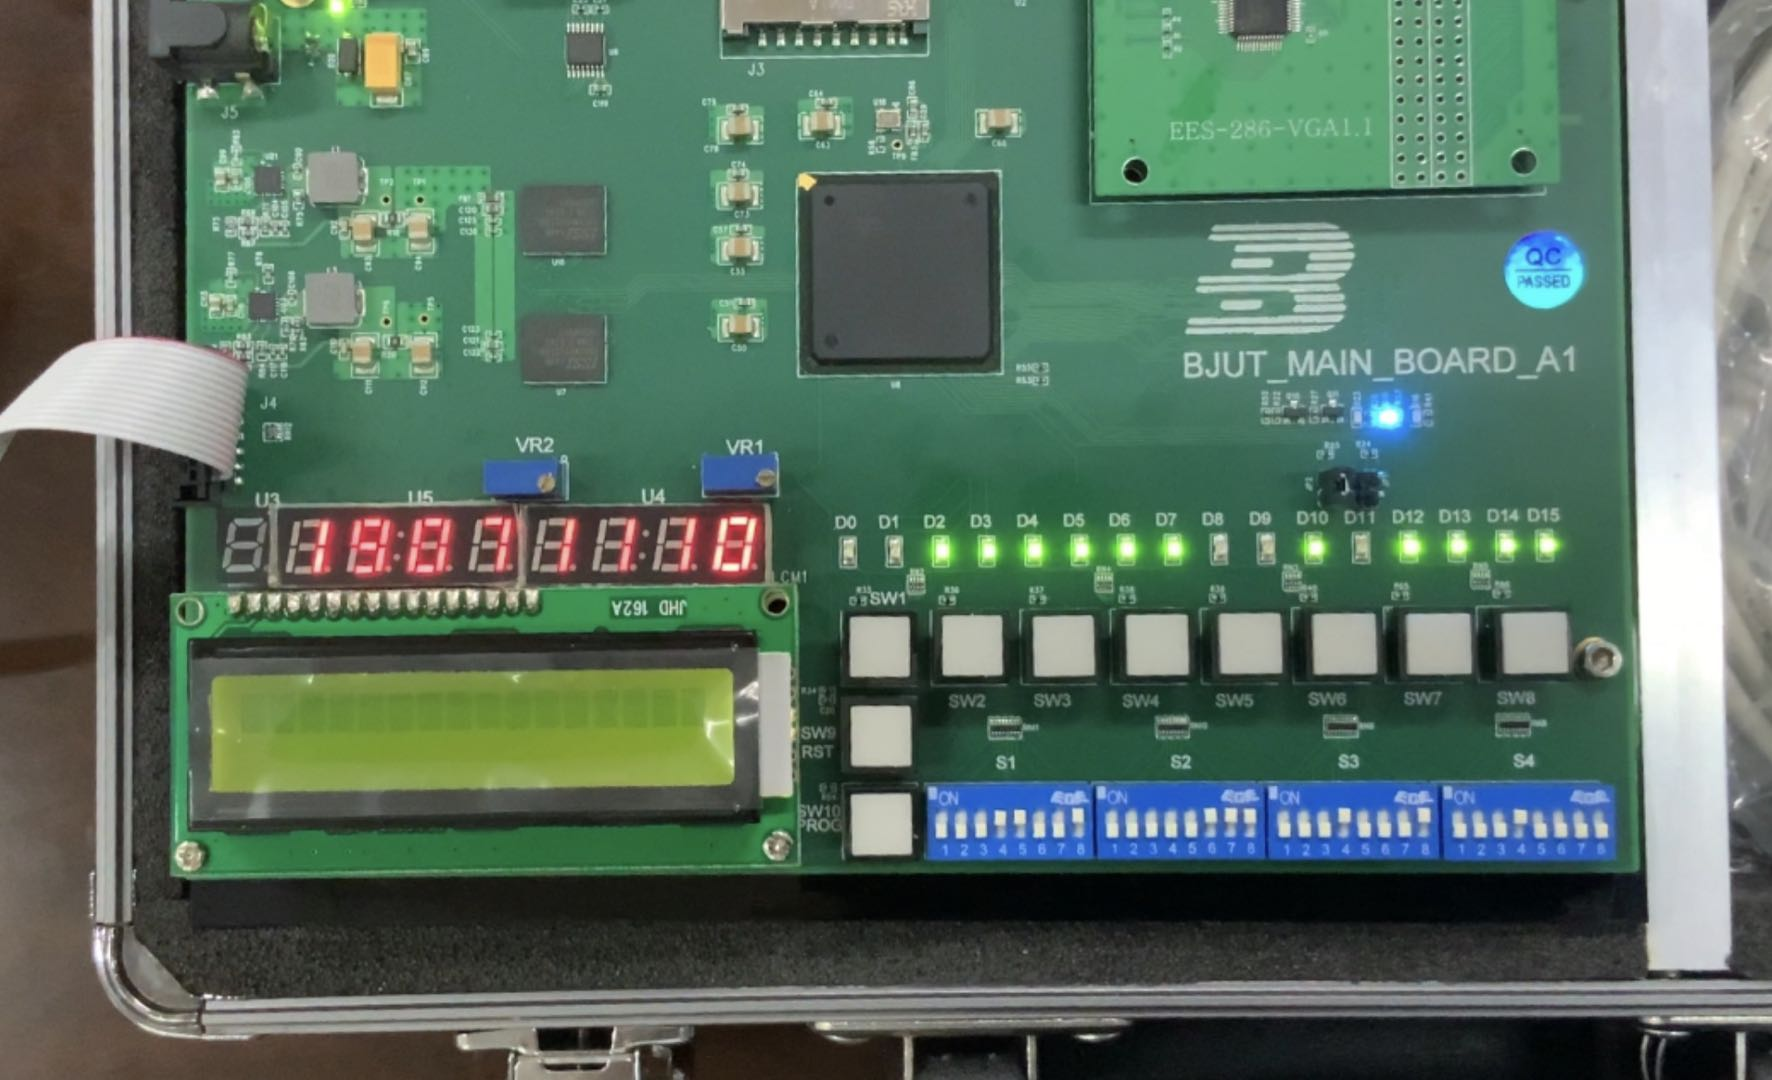
\includegraphics[width=\textwidth]{images/2MHz-set.jpg}
\caption{2MHz下正常运行-置数}
\end{figure}

\begin{figure}[h]
\centering
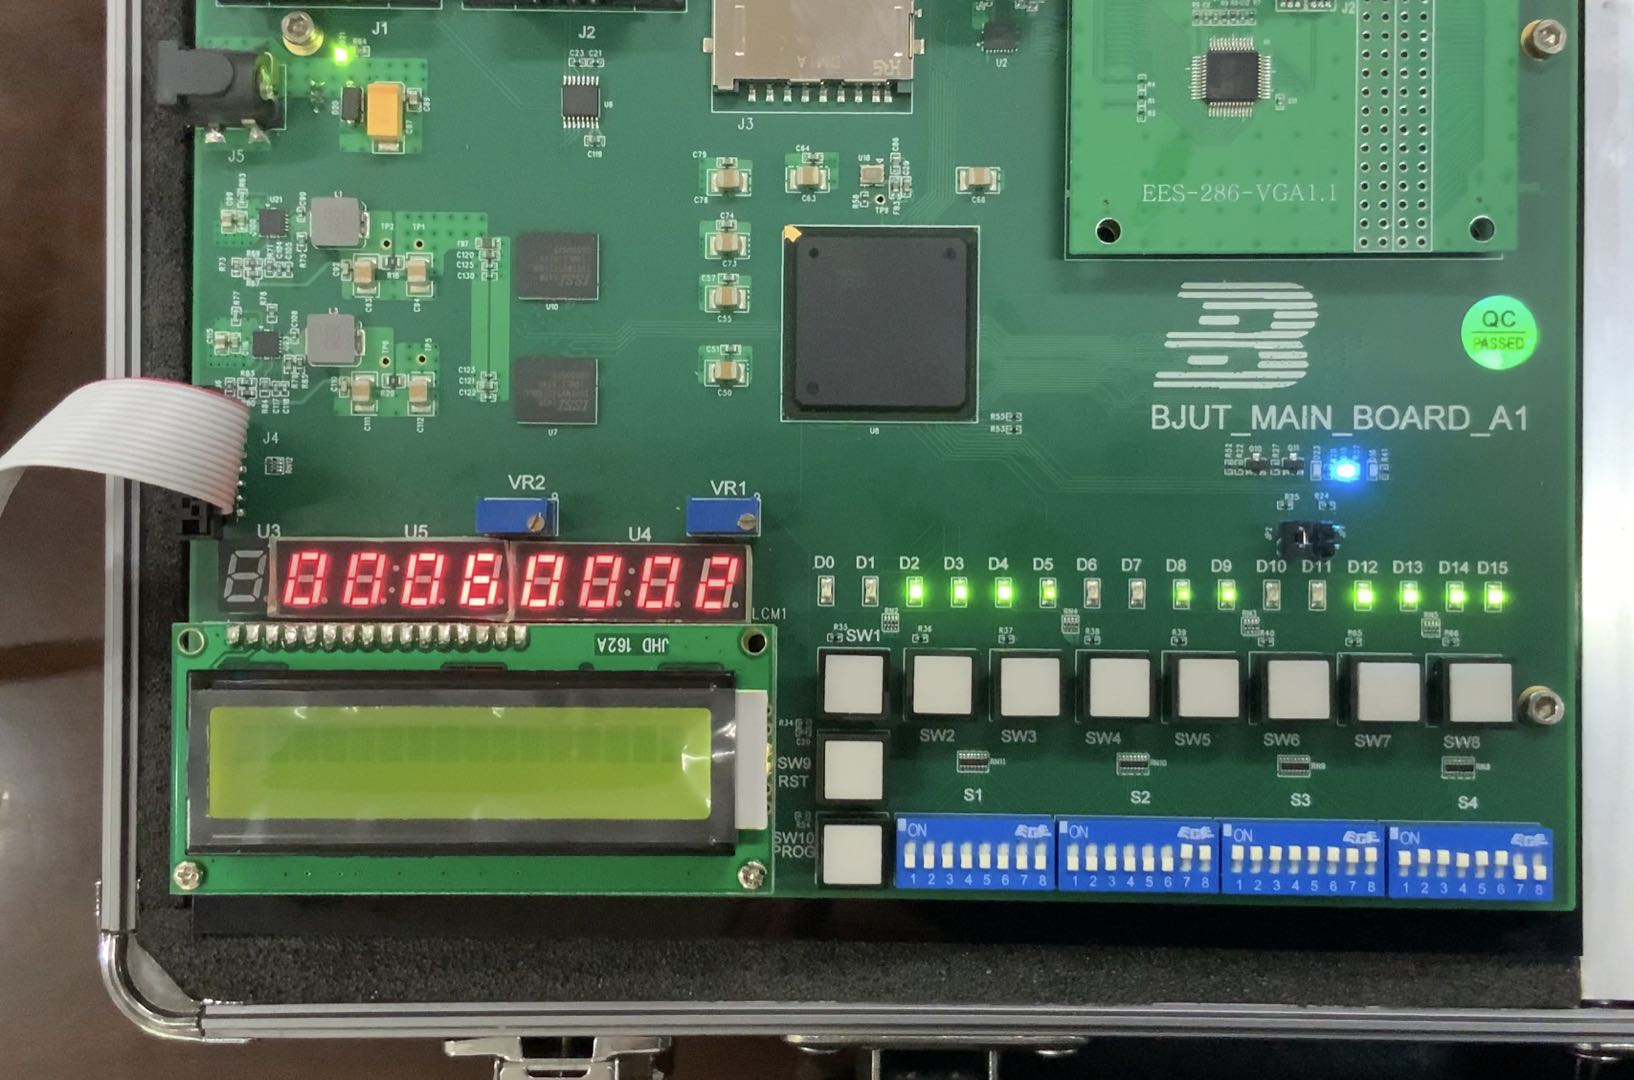
\includegraphics[width=\textwidth]{images/10MHz-error.jpg}
\caption{10MHz下出现错误}
\end{figure}

三张FPGA实验的图片中,前两张分别展示了CPU以2MHz主频运行时,可以正常实现计数、置数的功能。而最后一张在置数不久后拍摄,体现了10MHz下的问题(数码管本应显示0x0004\_0002却显示了0x0006\_0002)。



\subparagraph{整体总结} 测试结果与预期一致,验证了系统的工作正确性,且可以在主频最高$2MHz$下运行。

\end{document}
